\documentclass[a4paper]{article}
\usepackage[utf8]{inputenc}
\usepackage[bosnian]{babel}
\usepackage{graphicx}
\usepackage[colorlinks=true, allcolors=blue]{hyperref}
\usepackage{listings}

\title{
\huge Univerzitet u Tuzli\\
Predmet: Programski alati u tehničkom pisanju\\
Tema: Studentski biro}
\author{Majra Grabić}
\date{\today}

 

\begin{document}

\maketitle
\pagebreak
\tableofcontents
\pagebreak
\begin{abstract}
Moj rad predstavlja stranicu za organizaciju pod nazivom \emph{Studentski biro}. U nastavku predstavljeni su ciljevi projekta, sadržaj web stranica, ciljne grupe i slične web stranice. Takođe su opisane i tehničke karakteristike same stranice.
\end{abstract}

\section{Cilj projekta}
\subsection{Šta je Studentski biro?}
Projekat na kojem sam radila zove se \emph{Studentski biro}. To je web stranica na kojoj se zainteresovani studenti ali i srednjoškolci mogu prijaviti za rad od kuće kao freelanceri ili za rad u kompanijama koje traže honorarce u određenim gradovima. Ono što bi razlikovalo stranice za freelance i Biro je to da studenti dobiju određeni projekat na osnovu njihovih vještina koje posjeduju, a koje su naveli u svojoj prijavi, pa ga ne moraju tražiti sami. Takođe za početnike bi ovo bila mnogo pogodnija opcija od bilo kog drugog freelance sajta kako bi odmah na početku imali dobre satnice. 
Druga opcija Biroa jeste studentski rad kao honorarac u nekim firmama koje traže radnike, što bi mnogo olakšalo i poslodavcima i studentima koji traže posao. Satnice ili dnevnice su određene u ugovoru koje bi obje strane potpisale, a Biro bi od toga dobijao određeni procenat naknade zbog usluge. 

Kako sam spomenula da bi studenti napisali svoje vještine koje posjeduju u prijavu, željela bih napomenuti da to mogu biti vještine koje su ponuđene na stranici ili vještine koje bi oni dopisali u svojoj prijavi tačnije svom CV-u. Na osnovu toga, svakom bi studentu pronašli tačno ono što mu odgovara. Smatram da bi jedna ovakva organizacija, a samim tim i web stranica organizacije, zaista pomogla mnogima koji su u potrazi za poslom. Takođe ono što je najpogodnije jeste da se ne mora lično dolaziti u prostorije Biroa, nego bi se sve moglo završavati online putem, što bi itekako olakšalo, kako zbog situacije sa COVID-om, kako zbog zainteresovanih radnika ili poslodavaca koji su udaljeni od gradova u kojima se poslovnice nalaze. 

\subsection{Sadržaj web stranice}
Projekat se sastoji od četiri zasebne ali povezane html datoteke, na kojima se nalazi drugačiji sadržaj.

Na \emph{početnoj stranici} ideja je ukratko predstavljena na način da je opisana tačna lokacija Biroa, kratko je opisano ko se nalazi iza ideje, ali i to gdje studenti mogu raditi i kakve vještine im trebaju za rad. 

Na stranici \emph{o nama} nalazi se malo više informacija o samom birou, ali i poslovima koji su ponuđeni studentima. Takođe studenti su upoznati sa politikom Biroa, te da oni sami mogu zahtjevati od Biroa da im pronađe posao ukoliko se ne pronalaze u ponuđenim.

Na stranici \emph{kontakt}, nalaze se kontakt informacije, lokacije i radna vremena poslovnica po gradovima. Takođe na ovoj stranici nalazi se i forma za prijavu na Biro. 

Te na stranici \emph{poslovi} nalaze se prosječne dnevnice, ali i otvorena mjesta u gradovima u kojima su poslovnice, te online poslovi. 

\subsection{Zašto baš odabrati ovaj Biro?}
Na pitanje šta to radi ova stranica je već odgovoreno, ona pruža usluge zainteresovanim klijentima, bilo to poslodavcima ili radnicima - studentima. Sumirano, Biro povezuje dvije zainteresovane strane, osigurava obje putem ugovora koji se potpisuje i uzima određenu procentualnu naknadu za svoje usluge. 

Zajednici je Biro na raspolaganju prethodnih osamnaest godina no samo u Tuzli. Iz tog razloga je odlučeno da će se ciljna grupa povećati na sve studente iz BiH koji iskažu zainteresovanost za rad. Takođe ciljna grupa su i poslodavci koji žele honorarce ili freelancere. Upravo je to način doprinosa zajednici. Smatram da bi stranica bila vrlo posjećena jer je jedina na našem jeziku ovoga kalibra, koja bi bila u funkciji. Naravno postoji i konkurentska stranica \url{https://studentime.ba/} ali ne bavi se istim domenom rada. 

\section{Tehničke karakteristike}
\subsection{Broj stranica}
Kao što je već navedeno projekat je pravljen sa četiri odvojene html datoteke/stranice, koje su međusobno povezane ili putem navigacijske trake ili nekim drugim putem.


\subsubsection{Navigacijska traka}

\begin{lstlisting}[language=HTML]
        <nav>
 	  <a href="index.html" class="btn">Pocetna stranica</a>
 	  <a href="contact.html" class="btn">Kontakt</a> 
	  <a href="gallery.html" class="btn">Poslovi</a>
        </nav>
\end{lstlisting}
U prethodnom primjeru prikazan je model navigacijske trake na stranici \emph{o nama}. Klase koje su iste na sva tri linka su poslije korištene u CSS-u za dodavanje određenih tranzicija, boja i oblika. 

\begin{lstlisting}[language=HTML]
        <style>
        
	.btn:link,
        .btn:visited{
        
            margin-top: 200px;
            margin-bottom: 20px;
            display: inline-block;
            padding: 10px 30px;
            font-weight: 300;
            text-decoration: none;
            border-radius: 200px;
            transition: background-color 0.2s, border 0.2s, color 0.2;
            border 0.2s, color 0.2;
            background-color: #636e72;
            color: #fff;
            border: 1px solid #636e72;
            margin-right: 15px;
        }

            .btn:active,
            .btn:hover,
            .submit-btn:hover{
                border: 1px solid #b2bec3;
                background-color: #b2bec3;
            }
        </style>
\end{lstlisting}
Na ovaj način je u CSS fajlu uređena navigacijska traka koja se sastoji od tri linka u obliku dugmeta. Niti jedna stranica ne posjeduje dugme za nju samu. Navigacijska traka nalazi se na samome vrhu u header dijelu stranice, a iza nje je pozadinska slika koja je fiksirana. Takođe prikazan je i naziv klase submit-btn za dugme koje prijavnu formu šalje u dalju razradu, a nalazi se u body dijelu stranice \emph{contact.html}. 

\subsection{Funkcionalnost straica}

Svaka stranica ima drugačiju funkciju, a sa tehničke strane stranice se razlikuju jer je na \emph{gallery.html} prikazana tabela i recenzije studenata rađene uz pomoć JavaScript-a, na \emph{contact.html} je prijavna forma, na \emph{about.html} nalazi se video koji se reproducira kada je korisnik na stranici, a \emph{index.html} je glavna stranica koja prikazuje pozicije elemenata uz flexbox. Uz to, na svim stranicama nalazi se Pop-up dugme za chat, što će biti pojašnjeno u nastavku rada. 

\subsubsection{CSS}
U nekim slučajevima korišten je flexbox u CSS-u, a u nekim grid.
\begin{lstlisting}[language=HTML]
        <style>
        .main{
            display: flex;  
            flex-flow: row wrap;
            font-weight: bold;
            text-align: center;
            justify-content: space-between;
          }
          //prikaz CSS-a uz pomoc flexbox-a
          
          .row {
                zoom: 1;
            }
            
           .row:before,
           .row:after {
                content:"";
                display:table;
            }
           .row:after {
                clear:both;
            }
            
           .col {
                display: block;
                float:left;
                margin: 1% 0 1% 1.6%;
            }
            
           .col:first-child { 
                margin-left: 0; 
            }
            
           @media only screen and (max-width: 480px) {
                .col { 
                    margin: 0;
                }
            }
           .span-1-of-3 {
                width: 32.26%; 
            } //prikaz uz pomoc grid-a
        </style>
\end{lstlisting}
Što se tiče samog CSS koda, on je rađen bez template-a.

\subsubsection{JavaScript}
Dijelovi stranice rađeni u JavaScriptu su rađeni uz pomoć odgovarajućeg template-a koji je naveden u nastavku. Jedan od njih je prikazan:

\begin{lstlisting}[language=HTML]
<script>
        
 function openForm() {
  document.getElementById("myForm").style.display = "block";
}

function closeForm() {
  document.getElementById("myForm").style.display = "none";
}
</script>

<body>
<div class="chat-popup" id="myForm">
    <form action="/action_page.php" class="form-container">
    <label for="msg"><b>Message</b></label>
    <textarea placeholder="Type message.." 
    name="msg" required></textarea>
    
    <button type="submit" class="btn">Send</button>
    <button type="button" 
    class="btn cancel" onclick="closeForm()"> Close</button>
  </form>
</div>
</body>
\end{lstlisting}

U prethodnom primjeru prikazan je primjer za Pop-up chat preuzet sa \url{https://www.w3schools.com/howto/howto_js_popup_chat.asp}. 

Osim toga za recenzije studenata primjer je takođe preuzet sa \url{https://www.w3schools.com/howto/howto_js_quotes_slideshow.asp}

\subsubsection{Slike}
Slike koje su korištene nalaze se u folderu \emph{images}, a ovdje ću prikazati samo jednu, pozadinu header dijela index.html stranice. 

\begin{figure}[htp]
    \centering
    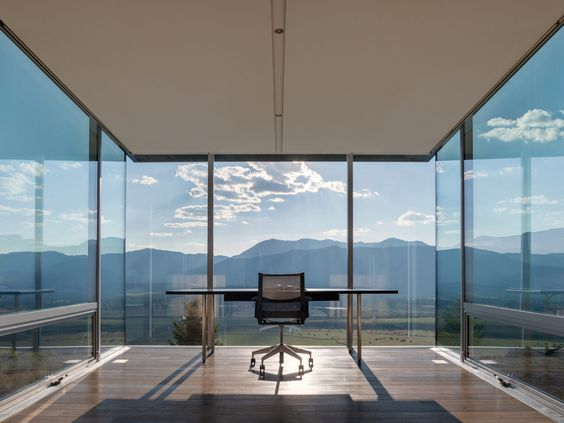
\includegraphics[width=8cm]{slika2}
    \caption{Naslovna slika}
    \label{fig:my_label}
\end{figure}

\subsection{Test rada stranice}
Stranica je testirana na tri Browser-a i to Google Chrome, Mozila Firefox i Microsoft Edge. Smatram da se ova tri pretraživača koriste najčešće te sam iz tog razloga odlučila svoje istraživanje o funkcionalnosti stranice provesti na njima.\cite{citiraj} 

\bibliographystyle{plain}
\bibliography{novabib}
\end{document}
